\section{Appendix}

\subsection{Mean face}
\begin{figure}
	\centering
	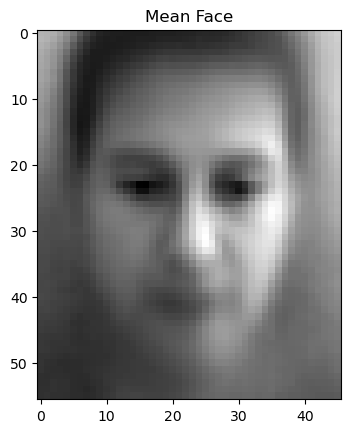
\includegraphics[width=0.4\linewidth]{image/q1_meanface.png} % Seems better to move to Appendix,,
	
	\caption{Mean face of training data}
	\label{fig:q1_meanface}
\end{figure}

\subsection{Confusion matrix}
\begin{figure}
	\centering
	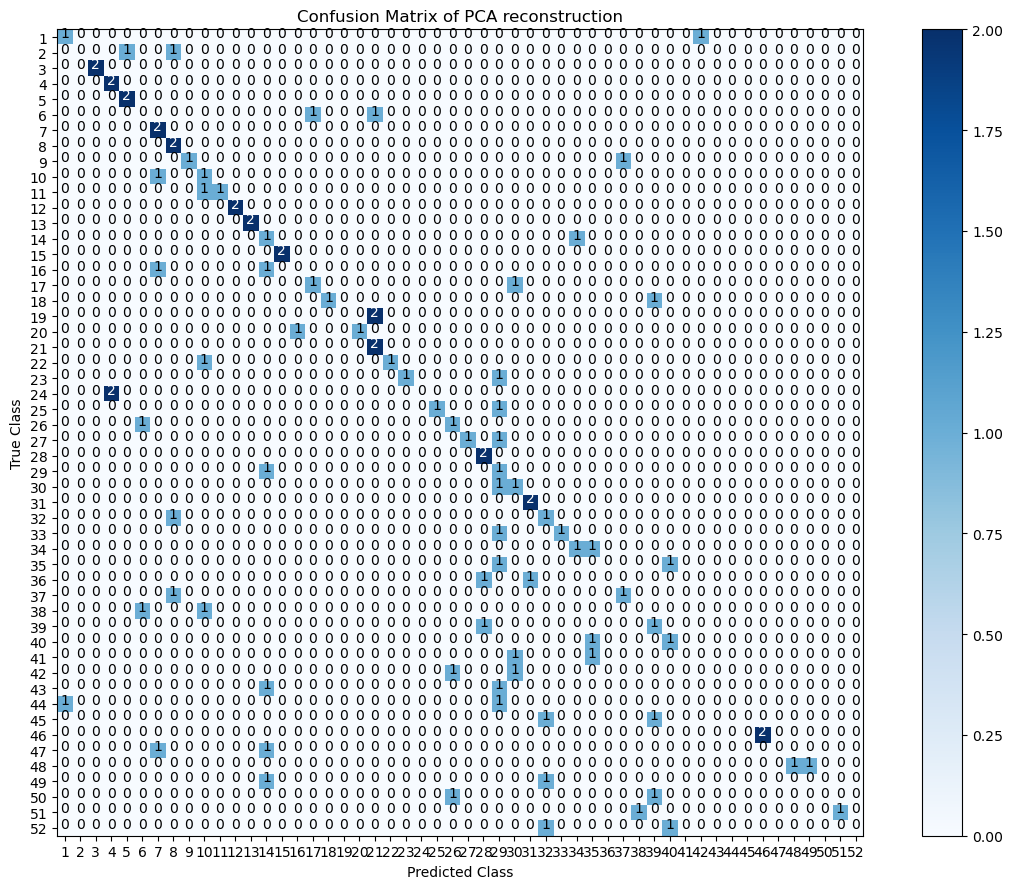
\includegraphics[width=0.4\linewidth]{image/q1_cm.png} % Seems better to move to Appendix,,
	
	\caption{Confusion matrix of PCA}
	\label{fig:q1_cm}
\end{figure}

\begin{figure}
	\centering
	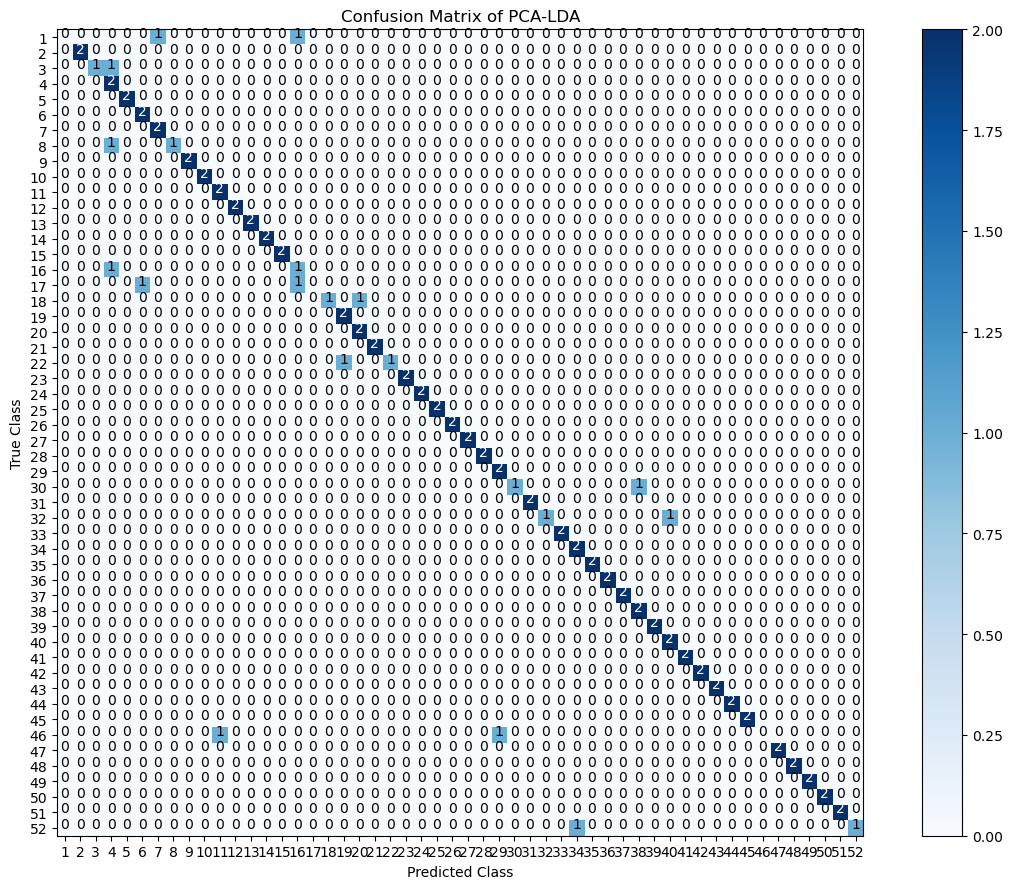
\includegraphics[width=0.8\linewidth]{image/q3_1_cm.png} % Seems better to move to Appendix,,
	
	\caption{Confusion matrix of PCA-LDA}
	\label{fig:q3_1_cm}
\end{figure}

\begin{figure}
	\centering
	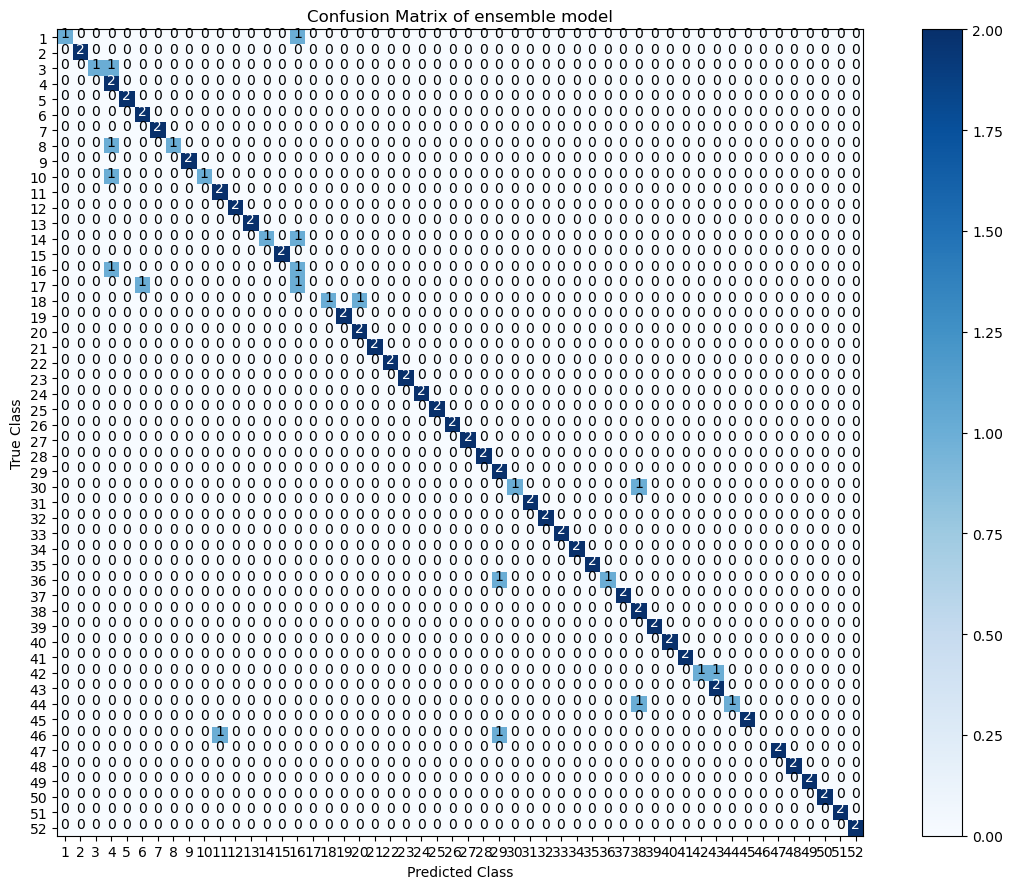
\includegraphics[width=0.8\linewidth]{image/q3_2_cm.png} % Seems better to move to Appendix,,
	
	\caption{Confusion matrix of Ensemble model}
	\label{fig:q3_2_cm}
\end{figure}

%-----

\subsection{Prediction examples}
\begin{figure}
	\centering
	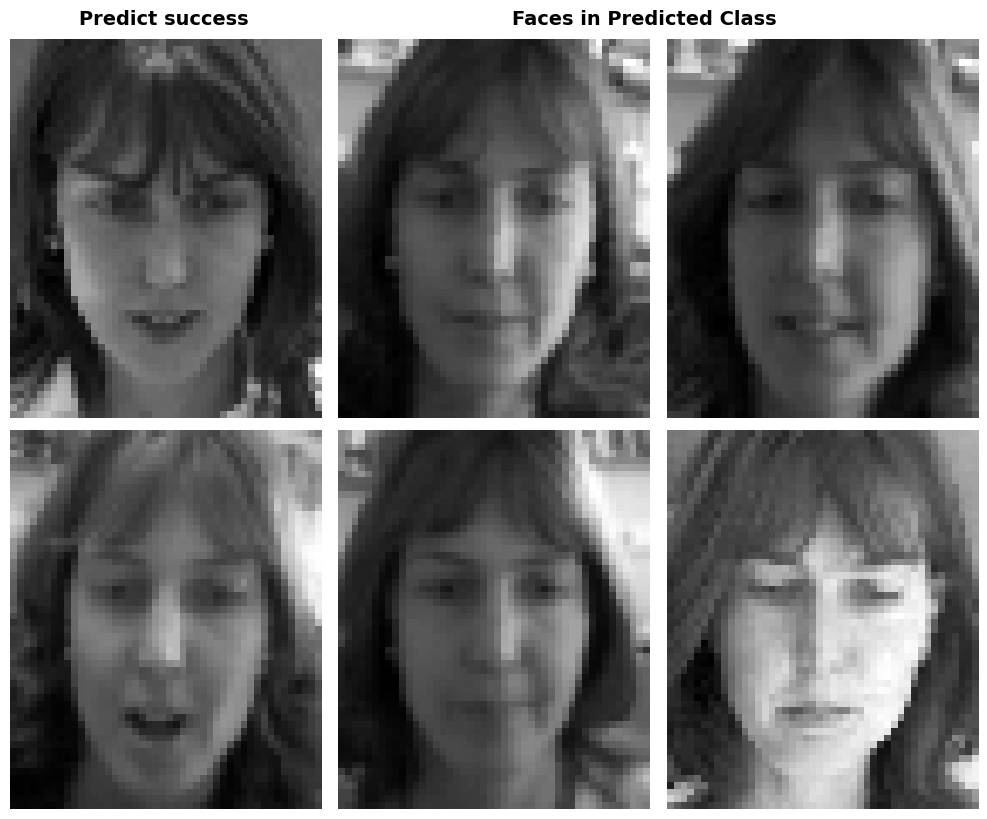
\includegraphics[width=0.8\linewidth]{image/q1_success.png}
	
	\caption{PCA classification success example}
	\label{fig:q3_success}
\end{figure}

\begin{figure}
	\centering
	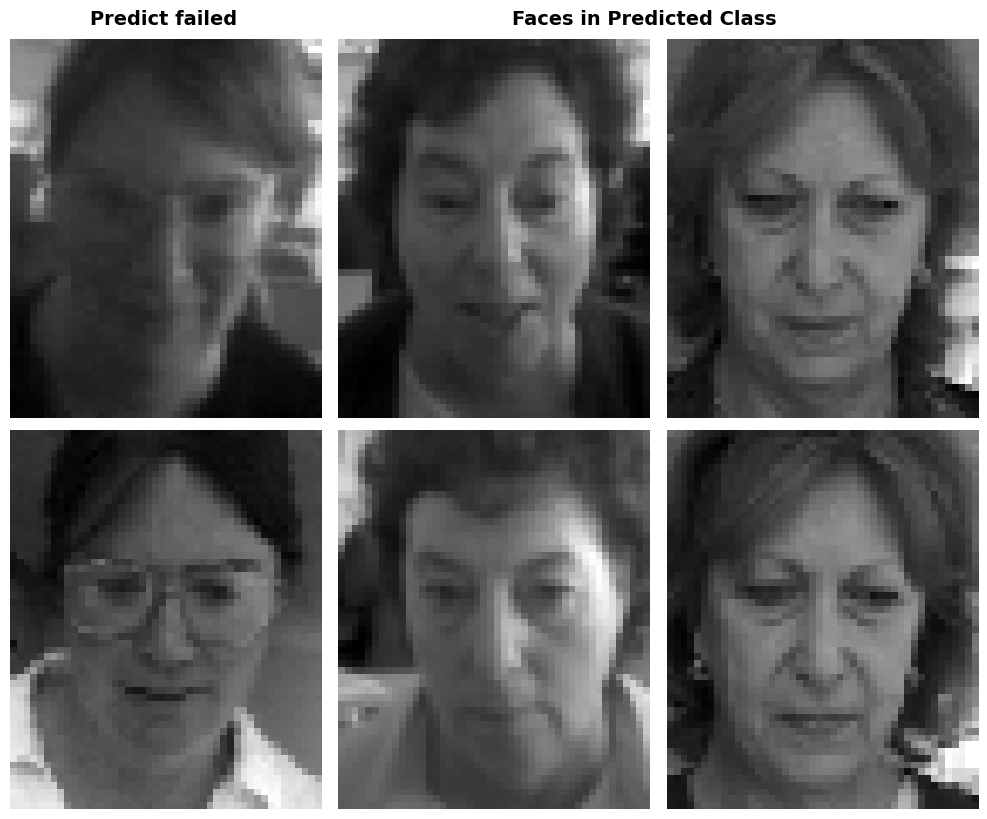
\includegraphics[width=0.8\linewidth]{image/q1_fail.png}
	
	\caption{PCA classification failure example}
	\label{fig:q3_fail}
\end{figure}

\begin{figure}
	\centering
	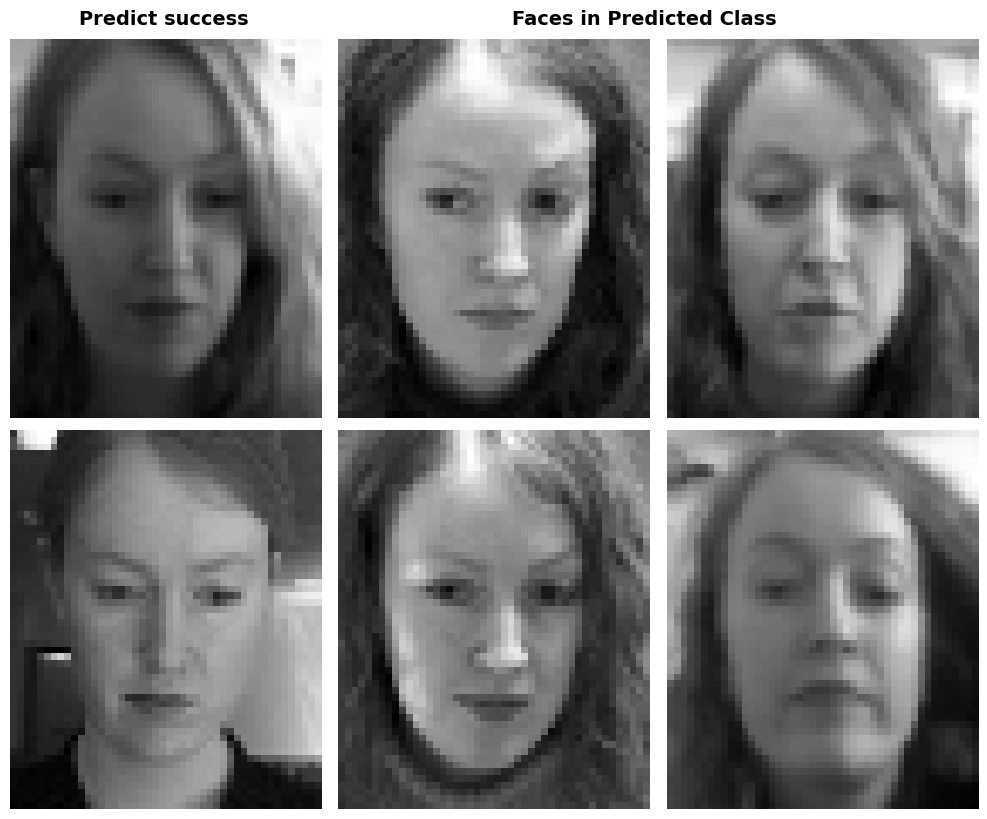
\includegraphics[width=0.8\linewidth]{image/q3_success.png}
	
	\caption{PCA-LDA classification success example}
	\label{fig:q3_success}
\end{figure}

\begin{figure}
	\centering
	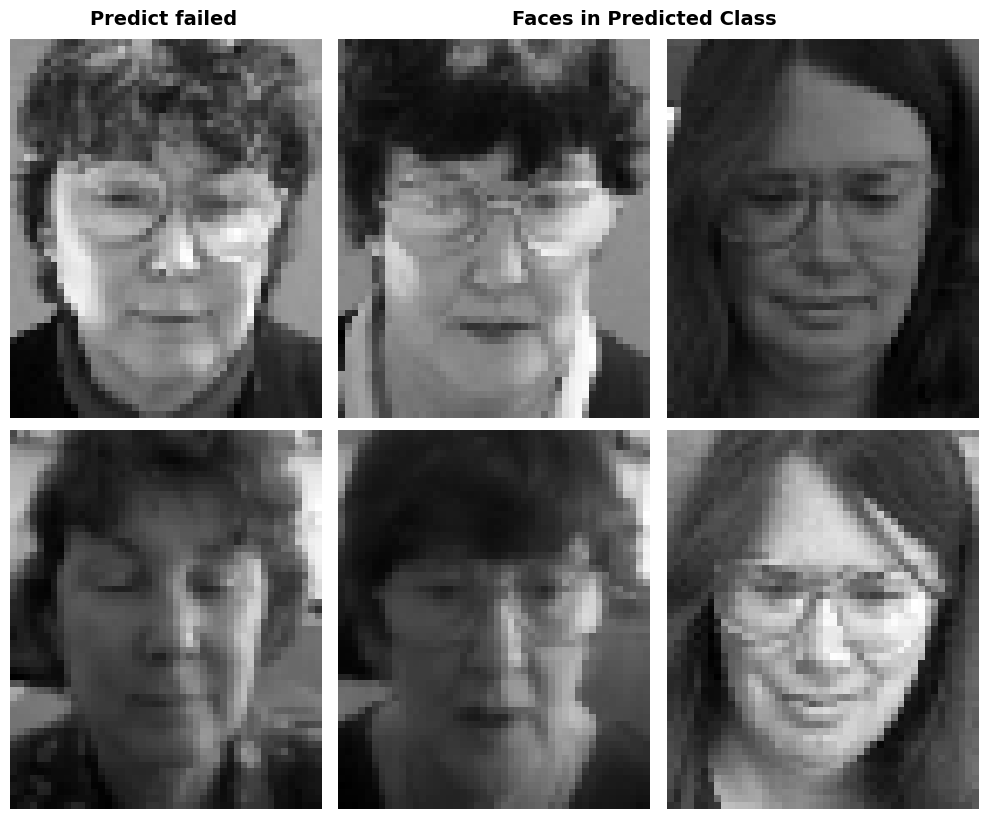
\includegraphics[width=0.8\linewidth]{image/q3_fail.png}
	
	\caption{PCA-LDA classification failure example}
	\label{fig:q3_fail}
\end{figure}

\subsection{Generative and Discriminative Subspace Learning}
\label{sec:intro}
Below is the objective function for generative and discriminative subspace learning. Our goal is to find $W$ that maximizes $J(W)$
\begin{equation}
	J(W) = \alpha W^TSW+(1-\alpha) \frac{W^TS_bW}{W^TS_wW}
	\label{eq:pca_lda_2}
\end{equation}
\cref{eq:pca_lda_2} can be changed as \cref{eq:pca_lda_3} since $W^TW=I$. (This is because, $W$ is a projection matrix, hence $W^TW$ indicates re-projection after projection to the subspace. Therefore, projected vector returns to itself after applying $W^TW$.)
\begin{multline}
	J(W) = \alpha \frac{W^TSW}{W^TW}+(1-\alpha) \frac{W^TS_bW}{W^TS_wW} \\
	= \frac{W^T(\alpha S + (1-\alpha)S_b)W}{W^T(\alpha I + (1-\alpha)S_w)W}
	\label{eq:pca_lda_3}
\end{multline}
If we keep the denominator constant, the problem we have to solve changes to the problem to maximize the numerator. Let the denominator $k(constant)$ and use Lagrange-multiplier. (\cref{eq:denominator})
\begin{equation}
	W^T(\alpha I + (1-\alpha)S_w)W = k
	\label{eq:denominator}
\end{equation}
\begin{multline}
	L(W,\lambda)=W^T(\alpha S + (1-\alpha)S_b)W \\
	+ \lambda(k-W^T\alpha I + (1-\alpha)S_w)W)
	\label{eq:lagrange}
\end{multline}
To get the solution, each partial derivatives of $L(W,\lambda)$ with respect to $W$ and $\lambda$ must be 0.
\begin{multline}
	\frac{\partial L}{\partial W} = 2*W(\alpha S+(1-\alpha)S_b \\
	-\lambda(\alpha I+(1-\alpha)S_w))=0
	\label{eq:partial_W}
\end{multline}
\begin{multline}
	\frac{\partial L}{\partial \lambda} = k - W^T(\alpha I+(1-\alpha)S_w)W=0
	\label{eq:partial_lambda}
\end{multline}
\cref{eq:partial_lambda} is satisfied from our assumption of the denominator. Now, the only thing we have to consider is \cref{eq:partial_W}. If we organize \cref{eq:partial_W}, we can get \cref{eq:solution}.
\begin{equation}
	(\alpha S+(1-\alpha)S_b)W = \lambda (\alpha I + (1-\alpha)S_w)W
	\label{eq:solution}
\end{equation}
If $\alpha I + (1-\alpha)S_w$ is invertible, the equation becomes as below.(\cref{eq:final})
\begin{equation}
	(\alpha I + (1-\alpha)S_w)^{-1}(\alpha S+(1-\alpha)S_b)W = \lambda W
	\label{eq:final}
\end{equation}
Since $\lambda$ is some constants, we can regard \cref{eq:final} as a eigenvector-eigenvalue problem where W is an eigenvector matrix and lambda is an eigenvalue matrix.

\subsection{Q5: Test result's confusion matrix and success/failure cases }
\label{subsec:Q5-1}
The optimal parameters determined for the random forest through experiments are $N=250$, $D=8$, and $\text{splitnum}=10$. With this configuration, each real-time executable weak learner—axis-aligned and two-pixel tests—each was trained 10 times. The confusion matrix results below represent the best test accuracy among the 10 repetitive train results.

\begin{figure}[h]
	\centering
	\begin{subfigure}[t]{0.4\linewidth}
		\centering
		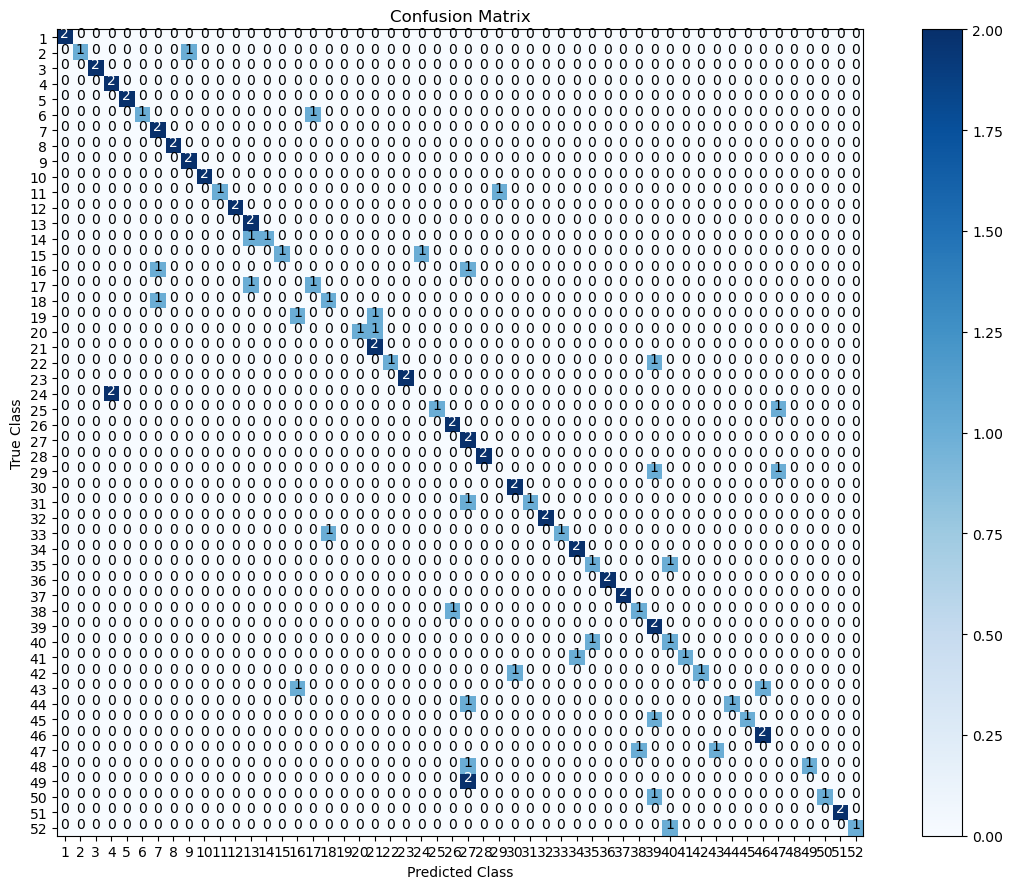
\includegraphics[width=\linewidth]{image/q5-fig6.png}
		\caption{Axis-aligned weak learner, test accuracy=0.644}
		\label{fig:q5-fig6}
	\end{subfigure}%
	\quad
	\begin{subfigure}[t]{0.4\linewidth}
		\centering
		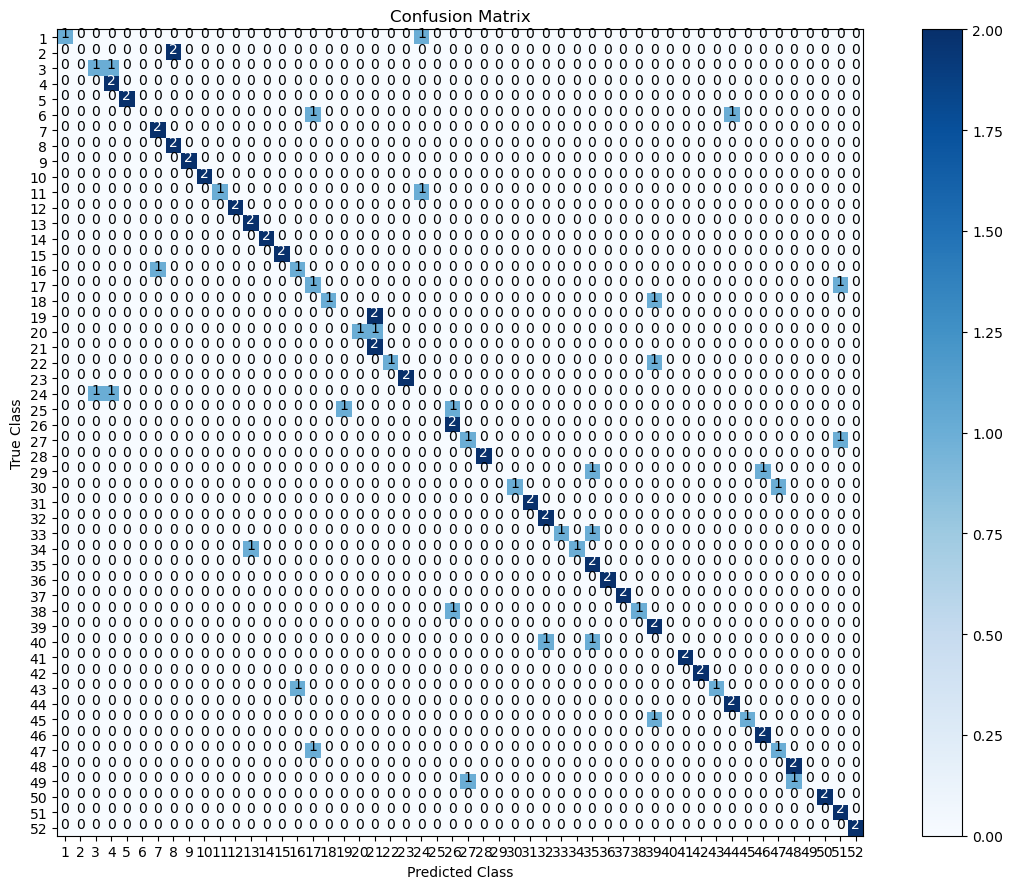
\includegraphics[width=\linewidth]{image/q5-fig8.png}
		\caption{Two-pixel test weak learner, test accuracy=0.692}
		\label{fig:q5-fig8}
	\end{subfigure}
	\caption{Confusion matrix of optimal cases ($N=250$, $D=8$, and $\text{splitnum}=10$)}
\end{figure}

Additionally, the example success and failure cases based on the confusion matrix results above are shown below. Compared to the success cases, the failure cases show a higher similarity between the failed image and the predicted class, meaning that our model is reasonable.
\begin{figure}
	\centering
	\begin{subfigure}{0.45\linewidth}
		\centering
		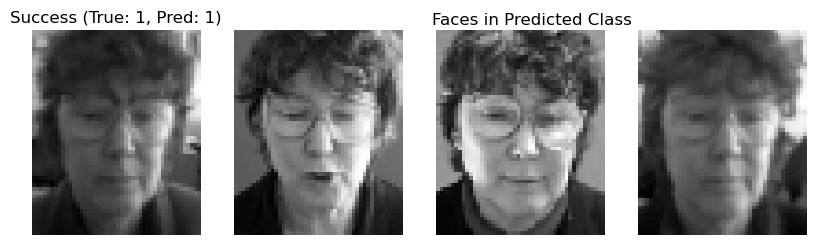
\includegraphics[width=\linewidth]{image/q5-app/q5-axis-succ1.png}
	\end{subfigure}%
	\quad
	\begin{subfigure}{0.45\linewidth}
		\centering
		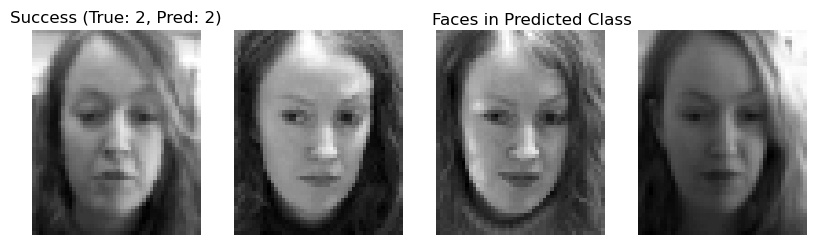
\includegraphics[width=\linewidth]{image/q5-app/q5-axis-succ2.png}
	\end{subfigure}
	\caption{Axis-aligned weak learner: Example success case}
\end{figure}
\begin{figure}
	\centering
	\begin{subfigure}[t]{0.45\linewidth}
		\centering
		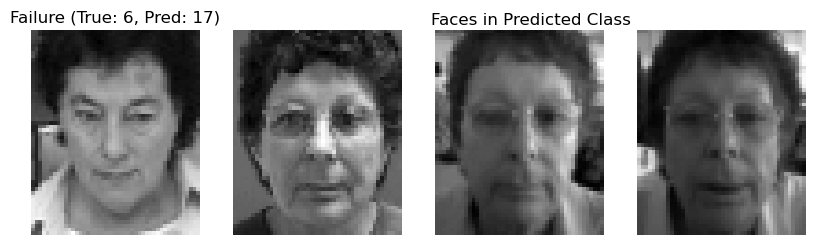
\includegraphics[width=\linewidth]{image/q5-app/q5-axis-fail1.png}
	\end{subfigure}%
	\quad
	\begin{subfigure}[t]{0.45\linewidth}
		\centering
		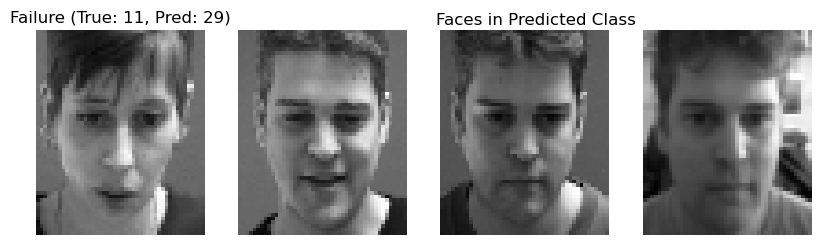
\includegraphics[width=\linewidth]{image/q5-app/q5-axis-fail2.png}
	\end{subfigure}
	\caption{Axis-aligned weak learner: Example failure case}
\end{figure}

\begin{figure}
	\centering
	\begin{subfigure}{0.45\linewidth}
		\centering
		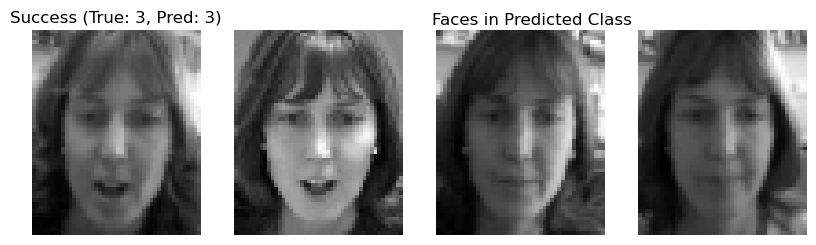
\includegraphics[width=\linewidth]{image/q5-app/q5-two-succ1.png}
	\end{subfigure}%
	\quad
	\begin{subfigure}{0.45\linewidth}
		\centering
		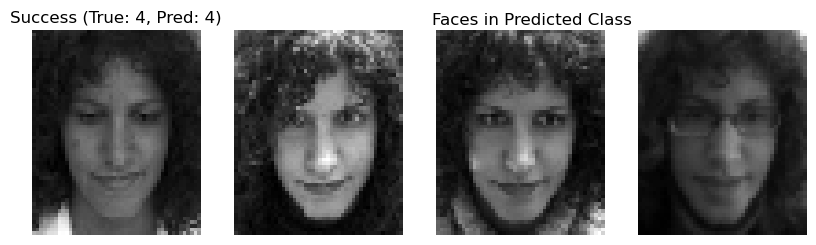
\includegraphics[width=\linewidth]{image/q5-app/q5-two-succ2.png}
	\end{subfigure}
	\caption{Two-pixel test weak learner: Example success case}
\end{figure}
\begin{figure}
	\centering
	\begin{subfigure}{0.45\linewidth}
		\centering
		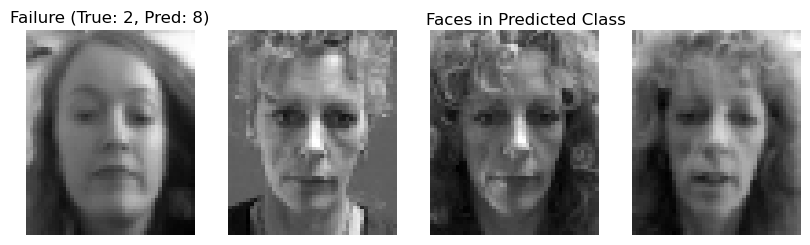
\includegraphics[width=\linewidth]{image/q5-app/q5-two-fail1.png}
	\end{subfigure}%
	\quad
	\begin{subfigure}{0.45\linewidth}
		\centering
		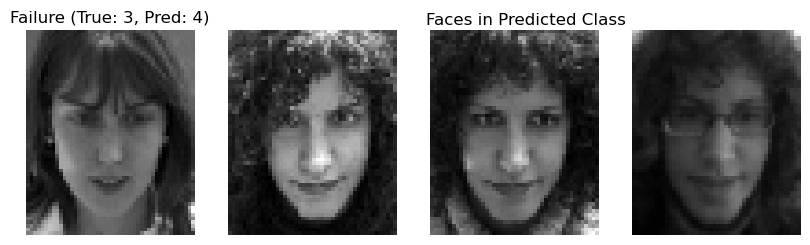
\includegraphics[width=\linewidth]{image/q5-app/q5-two-fail2.png}
	\end{subfigure}
	\caption{Two-pixel test weak learner: Example failure case}
\end{figure}

\subsection{Q5: Visualization of random forest's information gain process}
\label{subsec:Q5-2}